\chapter{基于流持续时间的传输优化方案}
\label{chapter:FDRC}
当前,许多应用(如网络搜索和零售)部署在数据中心。
由于TCP不能满足应用对延迟和吞吐量的需求,
因此研究者们提出了许多传输协议(例如,DCTCP,D$^2$TCP,L$^2$DCT)来对TCP进行补充。
其中,D$^2$TCP等协议将流的截止期限纳入拥塞窗口调整过程,以保证流在截止期限之前传输完成。
在数据中心中,短流常常需要较短延迟,因而,L$^2$DCT等协议在计算拥塞窗口调整因子时考虑流大小,以此保证短流的吞吐量和延迟。
这两种方法在一定的场景下运行良好,但依旧存在一些不足:
首先,这两种方法只能减小流错失期限的百分比或者能够减小流平均完成时间,但是不能够同时优化这两个目标。
其次,大多数方法都需要预知流的信息(例如截止期限,流大小),
但是对于很多应用,流大小以及流截止期限这些信息很难预先得知。
因此,在本章中,本文主张使引入流持续时间到拥塞窗口调整的过程中。
基于此,本文提出流持续时间速率控制机制(Flow Duration Time Rate Control,简称FDRC)。
本文发现,在不用预先得知流信息的情形下,FDRC可以减少流错失期限的比例并且能够减小流平均完成时间。
本章从理论上分析了FDRC的行为,并在ns-2和Iinux内核实现FDRC。
同时实验表明,在几乎所有场景下,FDRC比D$^2$TCP和L$^2$DCT的性能都要好。
平均来说,FDRC比基于期限的拥塞控制协议D$^2$TCP性能高30%,
比优化流平均完成时间的方法L$^2$DCT性能提高大约10% 。

\section{概述}
\label{FDRC:introduction}
如今,越来越多对延迟敏感的应用(例如网络搜索,零售)被部署在数据中心网络。
数据中心网络(DCNs)需要给应用提供高吞吐,低延迟的服务,此外还需要能够承受高并发等特殊需求。
最近,在这些需求中,延迟引起了更多的关注,因为这会影响用户在这些应用中的体验,从而影响收入。
事实上,对于数据中心应用,每增加100ms,可能导致$1\%$的收入损失\cite{DCTCP,LPD}。


特别的,数据中心的流是由长的背景流,对时延敏感的流和带宽敏感流的混合,使用TCP不能满足所有流的需求,
会导致下面的两个问题。
首先,使用TCP协议,会导致交换机缓冲区溢出,数据包重传,进而使的网络延迟加大,从而影响用户体验。
其次,网络发生拥塞时,TCP发送端拥塞窗口会减半,导致网络震荡严重,链接利用率低。
由于存在TCP以上不足,DCTCP\cite{DCTCP}被提出。 
DCTCP采用大多数现代交换机支持的ECN标记机制\cite{DCTCP},
首先在交换机上设置一个阈值K,当交换机缓冲区队列超过K时,发送到交换机的数据包会标记CE,
接收端收到所有的数据包后,如果有被标记CE的数据包,那么回复给发送端的ACK就会被标记ECN。
最后发送端统计上一个RTT中收到的ACK被标记的ECN的比例,然后计算链路拥塞程度,最后根据拥塞程度调整拥塞窗口。
DCTCP通过使的交换机缓冲区队列维持在较短水平上,从而可以减小排队延迟,同时可以维持高链路利用率。
但是,DCTCP不考虑流的期限问题,它对所有流都公平对待,这样会导致许多对延迟敏感的流错过期限\cite{D2TCP,D3}。
针对此,业界提出两类方法来弥补TCP的不足:

\textbf{(1)给流设置显式的期限。} 
例如D$^3$\cite{D3},D$^2$TCP\cite{D2TCP}和LPD\cite{LPD}这几个方法是
从用户态给应用的数据流设置期限,数据流带宽由网络拥塞程度和期限共同决定。
截止期限近的数据流得到的带宽比期限远的流得到的带宽多,
因此,截止期限近的流和截止期限远的流都能在截止时间之前完成。
通过设置不同的截止期限,优化数据流的传输延迟。

\textbf{(2)将短流设置为高优先级。}
在数据中心网络中,短流常常承载交互等信息,因此往往需要低延迟。
所以PDQ \cite{PDQ},L$^2$DCT\cite{L2DCT}和pFabric \cite{pFabric}等试图将短流设置为高优先级,长流设置为低优先级,
并试图实现最短流优先策略(Shortest Job First,简称SJF)。
事实上,在单条瓶颈链路的场景下,
最短流优先策略是减小流平均完成时间的最优策略。
事实上,在多链路的情形下,
最短流优先策略也能达到较好的性能\cite{L2DCT,pFabric}。


事实上,这两种方法都试图把紧急的流设置更高的优先级,优化紧急流的延迟。
区别在于第一种方法是根据用户期望的延迟设置优先级,第二种是根据流的大小设置优先级。
两种方法都需要用户事先得知流信息。
具体的,如果使用第一类方法,需要事先得知流的截止时间;如果使用第二类方法,需要事先得知流大小。
另外,数据中心的流是延迟敏感流,带宽敏感流和长的背景流的混合,
第一类方法可以满足延迟敏感流的需求,第二类方法只是试图降低流的平均完成时间。
事实上,这两种方法都不能同时满足延迟敏感流,带宽敏感流和长的背景流的需求,
所以这些方法在部署上有一定的局限性。

由于以上提到的缺陷,本文提出流的优先级可以根据流启动的持续时间来设置。
流在开始发送时具有最高优先级,随着时间的推移其优先级下降。
 一方面不需要事先知道流的信息(流的大小或截止时间);
另一方面,这种方法间接给短流设置了更高的优先级,短流经常有期限限制,短流能获得较多的带宽,
进而能够在截止时间之前完成,同时优化了流的平均完成时间。
基于此,本章提出了基于流持续时间的速率控制算法(Flow Duration Rate Control,简称FDRC)。
本章将FDRC实现在ns-2\cite{ns2}和Iinux 内核3.2.61上。
实验结果表明FDRC的性能比D$^2$TCP提高了$30\%$,比DCTCP提高了2$\times$。
本章中主要做了以下的工作:

(1)提出数据中心基于流持续时间的传输协议(Flow Duration Rate Control,简称FDRC)。
FDRC可以使更多流达到最终期限的限制,同时有助于减少流平均完成时间。
FDRC可以在事先不知道流信息的情形下,有效的减少流错过期限数目的百分比。

(2)在ns-2中评估FDRC,然后用DCTCP,D$^2$TCP,L$^2$DCT,LPD和pFabric与之对比。
最后,在linux内核中实现FDRC,并构建小型数据中心测试FDRC,进而评估FDRC的性能。


\section{相关工作和研究动机}
\label{FDRC:background}
\subsection{相关工作}

业界已经提出一系列方法来保证数据中心流传输延迟,
根据这些方法特性可以分为三类,第一类是基于TCP的方法,例如
DCTCP\cite{DCTCP},D$^2$TCP\cite{D2TCP}以及LPD\cite{LPD}等,
这类方法一般借助交换机ECN标记机制,通过ECN机制来评估交换机队列长度,
根据网络拥塞程度和流特性(期限,流大小)等进行速率控制;
第二类是网络调度方法,例如PDQ\cite{PDQ},D$^3$\cite{D3}等,
这类方法通常采用集中控制的方法,在此系统中,有一个集中控制器,
集中控制器需要预先得知网络的情形,根据网络实时拥塞状况对流进行调度;
第三类是控制交换机队列的方法,例如pFabric\cite{pFabric}等,
这类方法需要改动交换机队列,在交换机上实现特殊的队列控制机制,通过特殊队列进出方式,实现对流的速率控制。


以上的三类方法,无论是显式设置期限还是隐式的优化流完成时间,
都需要预知流的信息(流大小,截止期限,剩余流大小,剩余时间等)或者对网络设备进行修改。
但是在数据中心的流是混合了延迟敏感流,带宽敏感流和长的背景流。
给流设置截止期限,根据截止期限区分优先级,能够减少流错失期限的比例。
根据流大小进行调整,只能够优化流完成时间。
但是当前没有一种方法能够同时满足这两者的需求,此外这些方法还需要预先得知流信息。
实际需要一种无须知道流的信息就能够优化有截止期限的流和流完成时间。

\subsection{研究动机}\label{fdrc_motivation}

\begin{figure}[h]
\centering
\subcaptionbox{错失期限流比例}
 {\includegraphics[width=0.32\columnwidth]{figures/FDRC/motivation/miss_deadline.eps}}
\subcaptionbox{流平均完成时间}
{\includegraphics[width=0.32\columnwidth]{figures/FDRC/motivation/fct.eps}}
\subcaptionbox{背景流带宽}
{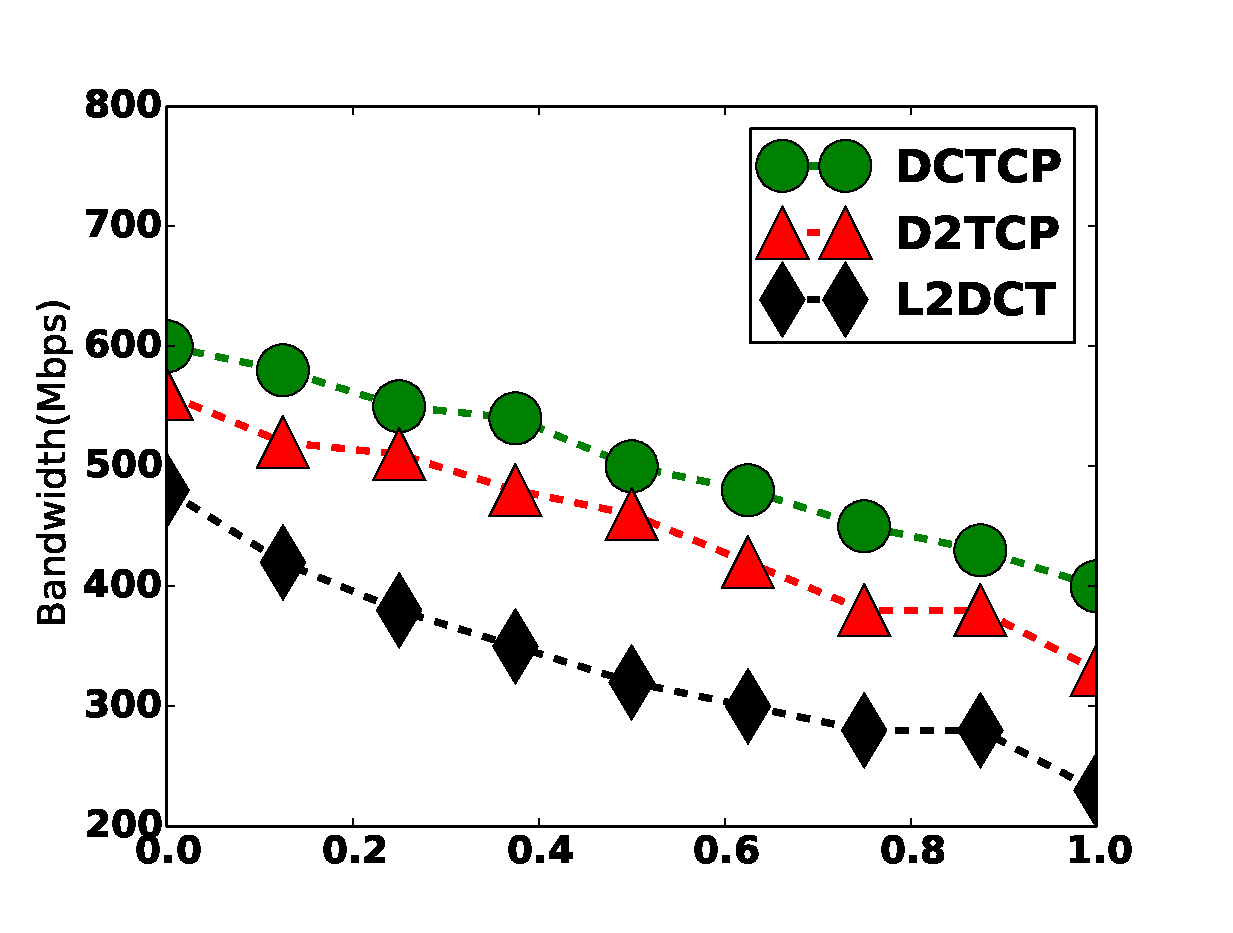
\includegraphics[width=0.32\columnwidth]{figures/FDRC/motivation/bandwidth.eps}}
\caption{研究动机: $50\%$的流有显式的期限,其他的流应该尽快的传输完}
\label{fdrc-motivation-fig}
\end{figure}

当前速率控制算法,无论是设定显式截止期限或者给短流设置高优先级,优化流平均完成时间,
可以使流在截止期限之前完成或减少流平均完成时间,但是不能同时满足两个目标。
为了验证此问题,在ns-2平台上,启动10个发送端,1个接收端,
它们共同连接到一个交换机上,设置交换机的缓冲区的阈值K$=25$。
实验中的所有链路均设置1Gbps的带宽,
在10个发送端中,有2个持续发送背景流,
另外8个不断发送大小从100KB到1MB的短流,将短流量平均分为两组:
对于第一组(4个发送端),期望短流能够在$30ms$之内完成传输(截止期限为30ms);
对于第二组(4个发送端),期望流平均完成时间尽可能短。
仿真时间持续10分钟,最终结果如图\ref{fdrc-motivation-fig}所示。

图\ref{fdrc-motivation-fig}(a)显示了几种方案下错失期限的流数目对比,
图\ref{fdrc-motivation-fig}(b)显示了流平均完成时间的对比。
图\ref{fdrc-motivation-fig}(a)所示,D$^2$TCP比L$^2$DCT 和DCTCP性能更好,
图\ref{fdrc-motivation-fig}(b)所示,对于流平均完成时间,L$^2$DCT性能更好。
这是因为使用D$^2$TCP,有显式期限的紧急流优先级较高,
从而获得较多的带宽,因而更有希望在截止时间之前完成。
但是,使用DCTCP和L$^2$DCT,第一组有期限的流与背景流的优先级相同,
因此很多期限近的流无法获得更多的带宽,从而会错失截止期限。
对于流平均完成时间,L$^2$DCT比D$^2$TCP性能更好,
这是因为在L$^2$DCT中,短流优先级高于长流,优先完成短流,
因此能够优化流平均完成时间,但是在实际中并不是所有的短流都有期限,
因而,对于有期限的流,L$^2$DCT并不能完全优化,所以,很多有期限的流并不能在截止时间之前完成。
图\ref{fdrc-motivation-fig}(c)显示了背景流的带宽。
可以看到,DCTCP下的背景流的带宽比D$^2$TCP与L$^2$DCT下背景流带宽高。


从图\ref{fdrc-motivation-fig}可以得出以下结论:
D$^2$TCP可以减少流错失期限的比例,L$^2$DCT 可以减少流平均完成时间。
但是,无论D$^2$TCP还是L$^2$DCT均不能同时满足这两个目标。
这是因为D$^2$TCP使用截止期限(deadline)作为速率控制因子,所以截止期限近的流将比截止期限远的流有更大的带宽。
但是D$^2$TCP无法优化流平均完成时间。
L$^2$DCT 使用流大小作为速率控制因子,因此小流将比长流有更高的平均带宽。
但是,在数据中心,并不是所有短流都有明确的截止期限(deadline),有些流只需要尽可能快的传输(例如小的请求)。
L$^2$DCT 将导致流平均完成时间较短,但是对于有显式期限的数据流会错失期限。

由于数据中心的流是有紧急期限的流,带宽敏感的流(希望流完成时间短)的混合,
所以需要一个协议来同时满足这两种流的需求。
当前无论D$^2$TCP或者L$^2$DCT均不能达到此目的,
它们只能优化有期限的流或者优化流完成时间,而无法同时满足两种需求。
因此,建议把流持续时间作为速率调整因子引入到流的速率控制中。
开始启动时,流具有最高优先级,随着时间流逝,流优先级下降。
引入流持续时间是一个很好的选择,
因为一方面这会使短流具有较高的平均带宽,
所以流有较短的平均完成时间;
另一方面,在固定时间阈值内的流将具有较大的平均带宽,
对于有期限的流也是一种较好的优化方法。


\section{FDRC策略}

\subsection{基于流持续时间的速率控制策略}

\begin{algorithm}
\KwIn{流启动时刻 $time\_start$,当前时刻  $time\_now$ }
\KwOut{窗口调整因子 $d$}
 $durtime=time\_now-time\_start$\;
  \If{durtime $\le threshold\_tight$}{
              $d=DMIN$\;
   }\ElseIf{durtime $\ge threshold\_lax$}{
   	  $d=DMAX$\;
   }\Else{
   d=$DMIN+\frac{(durtime-threshold\_tight)*(DMAX-DMIN)}{threshold\_lax-threshold\_tight}$
   }
   \textbf{return} d;
\caption{拥塞窗口因子计算算法}
\label{factor_algorithm}
\end{algorithm}

将流持续时间引入拥塞窗口控制,基于此,本文提出了基于流持续时间的策略(Flow Duration Rate Control,简称FDRC)。
算法\ref{factor_algorithm}展示了计算期限因子的步骤。
算法\ref{factor_algorithm}计算期限因子,需要四个参数: 
$threshold\_tight$和$threshold\_lax$是时间阈值,$DMAX$和$DMIN$是期限因子的上限和下限,当流的持续时间大于$threshold\_lax$时,
期限因子d被设置为$DMIN$,当流持续时间小于$threshold\_tight$,期限因子$d$被设置为$DMAX$。
当持续时间短于$threshold\_tight$时,流保持最高优先级。
如果流持续时间大于$threshold\_lax$,则流保持最低优先级。
对于$threshold\_tight$和$threshold\_lax$之间的流,优先级随着时间的推移而下降。
算法\ref{factor_algorithm}在每个RTT执行一次。
随着时间的推移,流优先级下降,因此,长的背景流的带宽平均值小于短流的带宽,流完成时间长。

\subsection{FDRC 协议}
FDRC基于DCTCP,在交换机端使用ECN标记模式。
交换机预先设置一个标记的阈值$K$。
当队列长度大于交换机的阈值$K$时,到达的数据包将被标记CE。
然后,接收端将检查来的数据包是否被标记,
如果发送过来的数据包有CE标记,则接收端回复的ACK中有ECN标记;
如果没有CE标记,那么接收端收到的ACK中没有ECN标志。
发送方每个RTT时间段,计算一下所有ACK中被标记ECN的比例,得到拥塞程度$\alpha$:
\begin{equation}
\label{alpha}
\alpha=(1-g) \times \alpha+g\times F
\end{equation}

其中,F是上一个RTT被标记ECN的比例。g是滑动平均的因子,拥塞程度$\alpha$反应的是这一段时间内的拥塞情况。
 根据计算的拥塞程度$\alpha$,得到FDRC拥塞窗口计算方法:
\begin{equation}
\label{factor}
f=\alpha \times d
\end{equation}

根据\cite{LPD},拥塞窗口的变化的加法增加部分和乘法减少部分可以是相同的。
根据此,改动滑动窗口的变化如下:
\begin{equation}
\label{ca}
 p=\left\{
\begin{array}{rcl}
w+(1-f)\\
w*(1-f) \\
\end{array} \right. 
\end{equation}


\subsection{FDRC 分析}
在本部分,从理论上分析FDRC的性能,建立两个模型来分析FDRC的性能:锯齿模型和FDRC-fluid模型。
锯齿模型是一个粗粒度的模型,FDRC-fluid模型是细粒度的模型。
本文使用锯齿模型用来分析FDRC速率和参数的关系,使用流模型,分析FDRC的参数。

\subsubsection{FDRC锯齿模型}
本部分建立锯齿模型\cite{LPD} 来分析FDRC的带宽。
$R_{1}$ 和 $R_{2}$ 表示 $flow_1$ 和 $flow_2$的速率。
假设两条流的拥塞窗口从$w_{min}$ 增加到 $w_{max}$,
有 $w^{av}=\frac{w_{min}+w_{max}}{2}$,其中$w^{av}$表示的是平均窗口大小。
流的拥塞窗口变化是有固定周期的锯齿,滑动窗口从$w_{min}$变化到$w_{max}$,需要N个RTT。
根据(\ref{ca}),滑动窗口每个RTT增加$(1-f)$,
因此得到最大的滑动窗口和最小滑动窗口的关系:$w_{max}=w_{min}+N \times(1-f)$。
当出现拥塞时候,窗口减小到$w_{min}$,
根据(\ref{ca}),有$w_{min}=w_{max}*(1-f)$。
令$w_{1}$是flow$_1$的最大窗口,
$w_{2}$是flow$_2$的最大窗口。
根据平均滑动窗口,计算两条流的平均发送速率比:
\begin{eqnarray}\label{fdrc-rate-ratio}
\frac{R_{1}}{R_{2}} =\frac{w^{av}_1}{w^{av}_2}
\end{eqnarray}
而 $w^{av}=\frac{w_{min}+w_{max}}{2}$,$w_{max}=w_{min}+N \times(1-f)$,带入(\ref{fdrc-rate-ratio}),得到二者的速率比:
\begin{eqnarray}\label{fdrc-rate-ratio2}
\frac{R_{1}}{R_{2}} &=&\frac{(2-f_1)\times w_1}{(2-f_2)\times w_2}  \nonumber \\
&=& \frac{2-\alpha d_1}{2-\alpha d_2}\times \frac{1-\alpha d_1}{1-
\alpha d_2}\times \frac{d_2}{d_1}\nonumber
\end{eqnarray}
当 $d_1$ 和 $d_2$ 很小,有$ \frac{2-\alpha d_1}{2-\alpha d_2}\simeq 1$,$ \frac{1-\alpha d_1}{1-
\alpha d_2}\simeq 1$,因此,可以得到:
\begin{equation}
\label{Ratio}
\frac{R_1}{R_2} \simeq \frac{d_2}{d_1}
\end{equation}

\begin{figure}[h]
\centering
\subcaptionbox{滑动窗口}
 {\includegraphics[width=0.48\columnwidth]{figures/FDRC/model/rate.eps}}
\subcaptionbox{队列长度}
{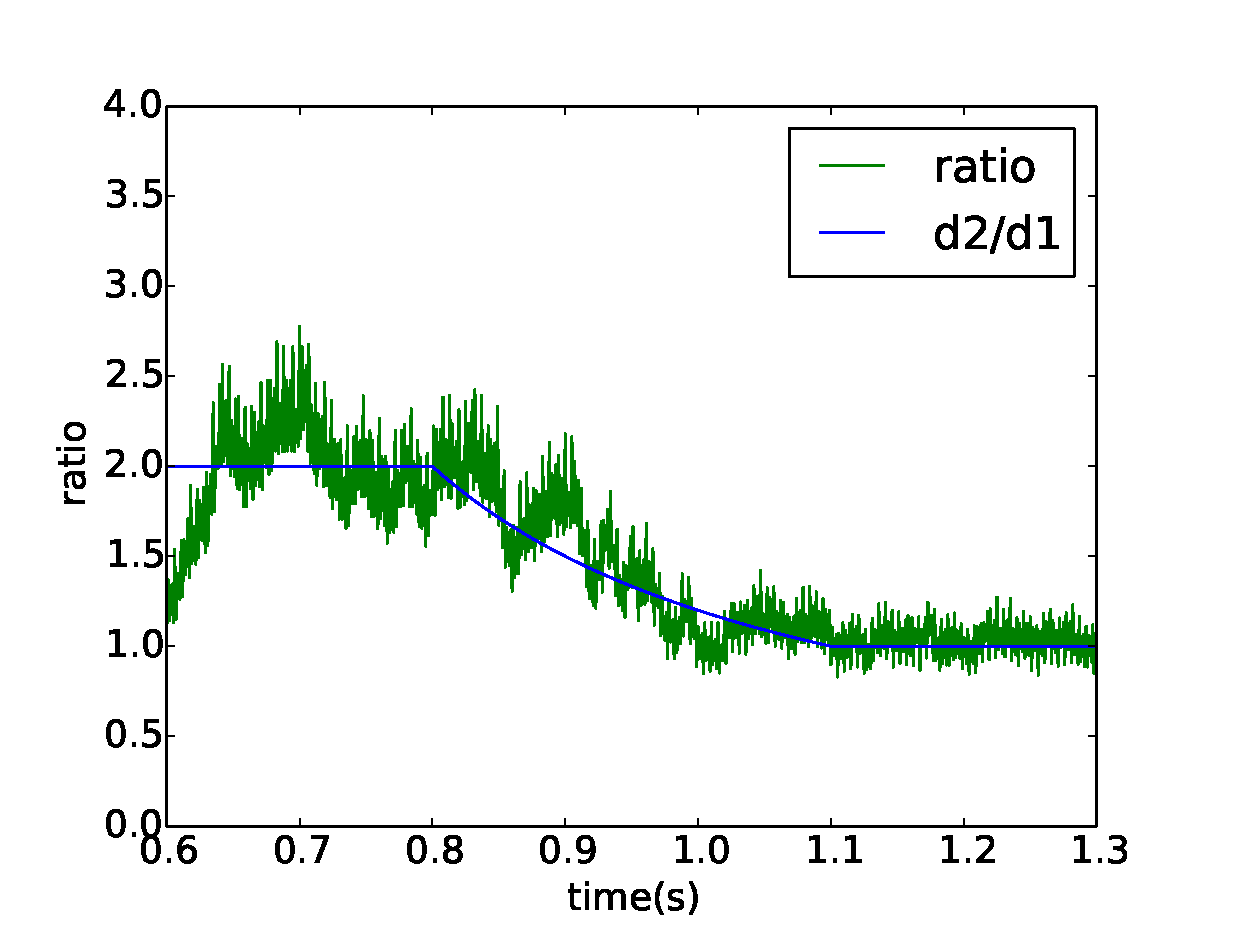
\includegraphics[width=0.48\columnwidth]{figures/FDRC/model/ratio.eps}}
\caption{(a) 显示了两条流带宽. (b) 显示二者的速率比和比例因子}
\label{fdrc-model-rate-ratio}
\end{figure}





从(\ref{fdrc-rate-ratio2})得知,对于两条流的窗口调整因子很小的场景,两条流的传输速率和窗口调整因子成反比。
为了测试模型的准确度,分别在t=0s和t=0.5s启动两条长流(其中flow$_1$的启动时间$start\_time = 0s$,flow$_2$的启动时间$start\_time = 0.5s$)。
设定阈值$threshold\_lax$ = 0.6s,阈值$threshold\_tight$= 0.3s,$DMIN = 0.05$,$DMAX = 0$。
当阈值$threshold\_lax$ = 0.6s时,flow$_1$从t = 0s开始,所以在$t = 0.6s$之后,flow$_1$的窗口调整因子$d= DMIN$。
$flow_2$从$t = 0.5s$开始,因此从$t = 0.5s$到$t = 0.8s$,窗口调整因子具有最大因子$DMAX$。
$t = 0.8s$后,窗口调整因子开始下降。
从$t = 1.1s$后,flow$_1$和flow$_2$具有相同的调整因子。

图\ref{fdrc-model-rate-ratio}(a)显示了两条流速率情形。
从图\ref{fdrc-model-rate-ratio}(a)可以看出,
从$t = 0.6s$到$t = 1.1s$,flow$_1$带宽大于flow$_2$,$t = 1.1s$后,两条流的带宽几乎相等。
图\ref{fdrc-model-rate-ratio}(b)显示了flow$_1$和flow$_2$的带宽比和因子比。
从$t = 0.6s$到$t = 0.8s$可以得知,两条流的因子比是$DMAX/DMIN = 2$,两条流的速率在此附近波动。
从$t = 0.8s$到$t = 1.1s$,两条流的窗口调整因子的比开始下降,两条流的速率比也在下降。
在$t = 1.1s$之后,两条流的调整因子比为1,两条流的带宽基本相同。

\subsubsection{FDRC流模型}
假设N个并发的流通过容量为C pkts / sec的瓶颈链路传递给同一个接收者节点,假设传输延迟为pd,
设置(\ref{Model-CA-eq})中$f_1(\alpha)=f_2(\alpha)=\alpha \times d$,
同时把$f_1(\alpha)$和$f_2(\alpha)$带入(\ref{fluid-model_window})$\sim$(\ref{fluid-model-q}),
并且改动(\ref{Model-alpha-eq})中数据包标记的方法,并且增加$\alpha$标记方法,那么FDRC-fluid模型可以描述为:

\begin{align}
&\frac{d\alpha_i}{dt}=\frac{g}{R(t)}(p(t-R^*)-\alpha_i(t)) \label{FDRC-model_alpha} \\
&\widehat{p}(t)=1_{\widehat{q}(t)>1}  \label{FDRC-model_mark} \\
&\frac{dq}{dt}= \sum_{i=1}^N{\frac{w_i(t)}{R(t)}}-C \label{FDRC-model_queue}  \\
&\frac{dw_i}{dt}=\frac{1-\alpha_i(t)\times d_{i}(t)}{R(t)}-\frac{w_i(t) \times \alpha_i(t)\times d_i(t)}{R(t)}p(t-R^*)  \label{FDRC-model_window}
\end{align}

\begin{figure}[h]
\centering
\subcaptionbox{滑动窗口}
 {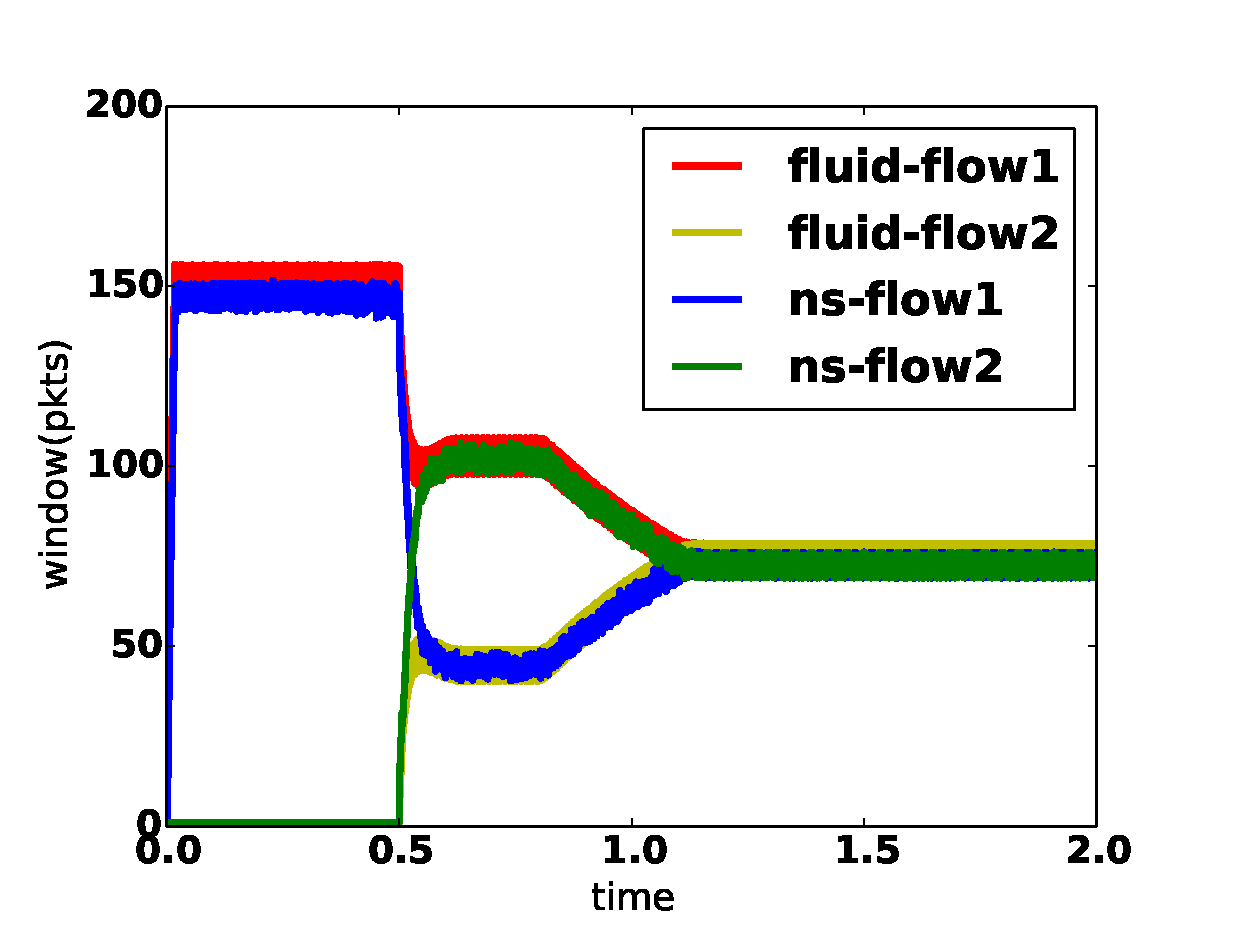
\includegraphics[width=0.32\columnwidth]{figures/FDRC/model/window.eps}}
\subcaptionbox{队列长度}
{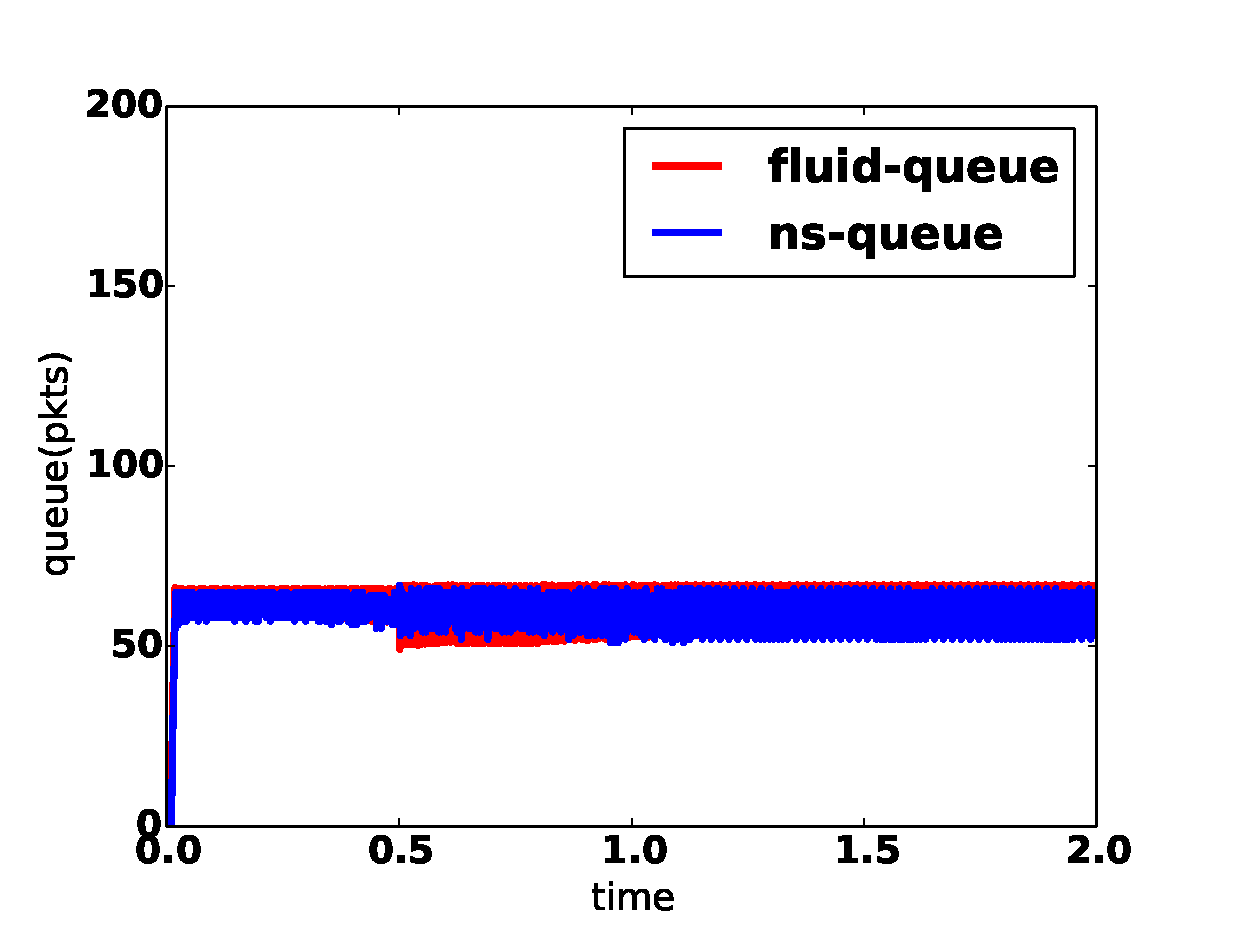
\includegraphics[width=0.32\columnwidth]{figures/FDRC/model/queue.eps}}
\subcaptionbox{$\alpha$}
{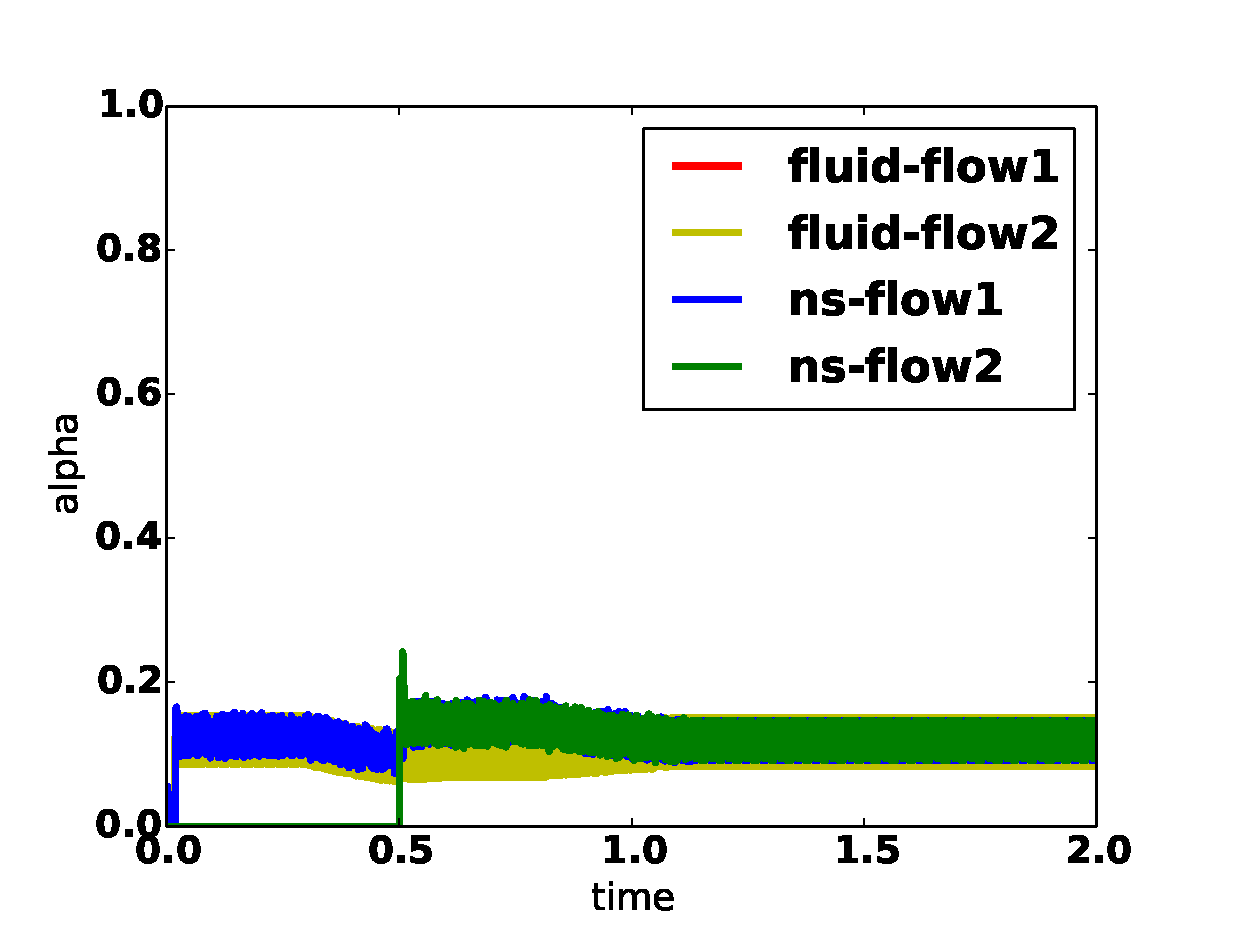
\includegraphics[width=0.32\columnwidth]{figures/FDRC/model/alpha.eps}}
\caption{FDRC的流模型推算结果和ns-2结果对比}
\label{fdrc-fluid-model-fig}
\end{figure}

等式(\ref{FDRC-model_mark})和等式(\ref{FDRC-model_queue})描述了交换机标记数据包的过程。
等式(\ref{FDRC-model_queue})描述了队列的长度,等式(\ref{FDRC-model_window})描述发送端窗口长度。
为了验证的模型,启动了两条长流(flow$_1$的启动时间$time\_start = 0s$,flow$_2$的启动时间$time\_start = 0.5s$)。
$DMAX = 1$,$DMIN = 0.5$,设置两个阈值:$threshold\_tight = 0.3s$,$threshold\_lax = 0.6s$。
对于持续时间小于0.3s的流,具有最大的调整因子值$DMAX$,对于持续时间大于0.6s的流,具有最小的调整因子值$DMIN$。
对于持续时间在0.3s到0.6s之间的数据流,调整因子在不断减小。
为了验证模型,使用FDRC模型来预测拥塞窗口并将FDRC-fluid模型推算结果与ns-2仿真结果进行比较。

图\ref{fdrc-fluid-model-fig}(a)描述了拥塞窗口的变化。
可以看到,起初只有flow$_1$开始,
所以flow$_1$占据了所有链路带宽,此时滑动窗口为150 MSS。
在$t = 0.5s$时,flow$_2$ 启动。
在$t = 0.5s$时,flow$_2$的因子大于flow$_1$,
所以flow$_2$拥有更大的拥塞窗口。
在$t = 1.1s$后,它们具有相同的拥塞窗口控制因子,
因此二者的滑动窗口开始逐渐相同。
图\ref{fdrc-fluid-model-fig}(b)显示了队列大小,
图\ref{fdrc-fluid-model-fig}(c)显示了流的拥塞程度$\alpha$。
可以看到,
对于流模型的队列长度和流的拥塞程度$\alpha$,
仿真结果和模拟结果基本相似。


\subsubsection{FDRC参数选取}
实际当中使用FDRC协议,有4个全局参数是必需的。
首先,两个时间阈值$threshold\_tight$和$threshold\_lax$可以根据实际应用的传输期限进行设置。
例如,在数据中心,数据流传输有截止期限,截止期限常常是一个时间范围,可以将$threshold\_tight$设置为期限的下界,
同时将$threshold\_lax$设置为期限的上界。
分析如何设置$DMIN$和$DMAX$。
首先,根据FDRC-fluid模型,得到不动点 ($w_i$,$\alpha_i$,q)=($\frac{1}{d_i}$-1,1,$\sum_{i=1}^N \frac{1}{d_i}-N-C\times pd$)。
不动点的物理含义是,所有发送到交换机的数据包都被标记CE,此时发送者窗口处于固定状态,不再发生变化。
在实际中,交换机队列不可能太大,因为较长的队列会导致较长的排队延迟。
在FDRC系统中,队列长度应该小于$K + N$,所以可以得到:
\begin{equation}
\label{queuelength}
\sum_{i=1}^N \frac{1}{d_i}-N-C\times pd \le K+N
\end{equation}
因为,在FDRC中,窗口调整因子d 在$DMIN$ 和 $DMAX$之间波动,因此对于d取得$DMIN$时,可以得到:
\begin{equation}
\label{DMAXvalue}
N \times \frac{1}{DMIN}-N-C\times pd \le K+N
\end{equation}

因此,得到:

\begin{equation}
\label{DMAXvalue}
DMIN \ge \frac{N}{2\times N +C \times pd +K}
\end{equation}
从 (\ref{ca}), 得知拥塞窗口控制函数$f<1$, 当 $\alpha \times d$ 到达1时,可以得到$d<1$,
因此$DMAX$ 和$DMIN$ 应该小于1。
$DMIN$和$DMAX$应该满足:
\begin{equation}
\label{DMAXDMIN}
\frac{N}{2\times N +C \times pd +K} \le DMIN < DMAX \le1
\end{equation}
在数据中心中,端和端之间的并发数往往小于100\cite{DCTCP},假定$C=10Gbps$,$pd=100us$,K设定为64,
数据包的大小设定为1500B,因此可以得到:
\begin{equation}
\label{DMAX_DMIN_RANGE}
0.29 \le DMIN < DMAX \le1
\end{equation}





\section{实验验证}
在本节中,在ns-2的平台和Linux真实测试环境下对FDRC的性能进行测试。
首先在仿真平台上,用实验发现FDRC可以解决动机部分\ref{fdrc_motivation}提出的问题。
之后,验证FDRC对流完成时间的优化,实验结果发现,对于流完成时间,FDRC比DCTCP降低了约$50\%$。
最后,在小型数据中心测试平台上评估FDRC的性能。

\subsection{解决研究动机提出的问题}
\begin{figure}[h]
\centering
\subcaptionbox{流错失期限百分比}
 {\includegraphics[width=0.32\columnwidth]{figures/FDRC/evaluation/spineleaf/miss_deadline.eps}}
\subcaptionbox{流平均完成时间}
{\includegraphics[width=0.32\columnwidth]{figures/FDRC/evaluation/spineleaf/fct2.eps}}
\subcaptionbox{流带宽}
{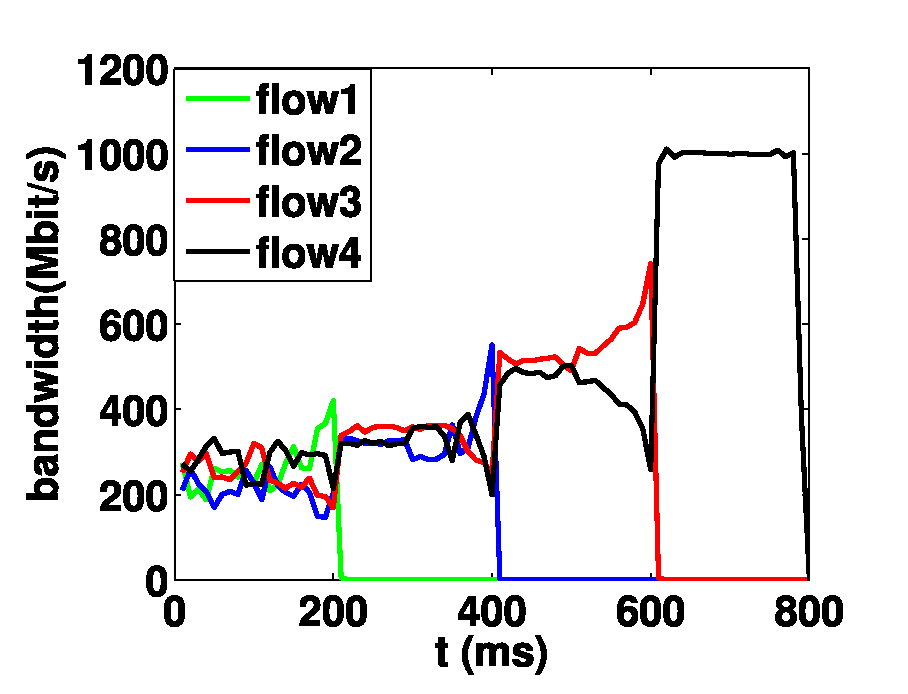
\includegraphics[width=0.32\columnwidth]{figures/FDRC/evaluation/spineleaf/bandwidth.eps}}
\caption{动机部分的例子:FDRC的性能和DCTCP,L$^2$DCT,D$^2$TCP性能的对比}
\label{fdrc-motivation-resolved-fig}
\end{figure}


在这一节中,首先解决动机部分\ref{fdrc_motivation}提出的问题。
对于FDRC,因为数据中心,流的期限通常在10ms至30ms之间,
因此在实验中,设置阈值$threshold\_lax$= 30ms,阈值$threshold\_tight$= 10ms。 
根据(\ref{DMAX_DMIN_RANGE}),可以设置 $DMAX = 0.8$,$DMIN = 0.3$。
对于DCTCP,D$^2$TCP,L$^2$DCT,以及其他的实验参数和实验环境,
使用和\ref{fdrc_motivation}相同的配置进行实验。


最终实验结果如图\ref{fdrc-motivation-resolved-fig}所示。
从图\ref{fdrc-motivation-resolved-fig}(a)看到,
总体上,几乎在所有情况下,使用FDRC时,流错失期限的比例比D$^2$TCP,L$^2$DCT,DCTCP更少。
相对于DCTCP,FDRC流错失期限的比例平均少$30\%$;
相对于D$^2$TCP,FDRC流错失期限的比例平均少$20\%$;
相对于L$^2$DCT,FDRC流错失期限的比例平均少$10\%$。
图\ref{fdrc-motivation-resolved-fig}(b)反应的是流平均完成时间对比结果,
从总计看,使用FDRC时,对流平均完成时间的优化是最好的。
对于流平均完成时间,FDRC比DCTCP平均小$30\%$,相比于D$^2$TCP,
FDRC性能好$20\%$,相比于L$^2$DCT,FDRC性能好$10\%$。
图\ref{fdrc-motivation-resolved-fig}(c)反映的是背景流带宽情形,
可以发现FDRC获取带宽的能力和L$^2$DCT基本相同,比D$^2$TCP和DCTCP要强。

分析FDRC能同时优化带有期限的数据流和优化流完成时间的原因。
首先,FDRC使用流持续时间作为滑动窗口的控制因子,在实验中,设置阈值$threshold\_lax$= 30ms,阈值$threshold\_tight$= 10ms,
所以期限在30ms以内获得的平均带宽高,
紧急流将比宽松的流更高的带宽,所以更少的流将错过最后期限。
由于刚开始启动时,流的优先级最高,随着时间的推移而下降,
所以短流的平均带宽比长流的平均带宽要大,
因而,FDRC近似实现短流优先策略,流平均完成时间小。

\subsection{真实流量和拓扑下仿真}

本部分用真实的数据中心流量和复杂的数据中心拓扑来测试FDRC的性能。
在ns-2中构建如图\ref{FDRC-DataCenterTop-fig}所示的Spine-Leaf拓扑。
在ns-2的仿真实验中,启动144个服务器,9个叶子交换机和4个主干交换机,其中9个叶子节点交换机和4个主干交换机相连接。
通过主干交换机(4跳)的端到端往返延迟是14.6us,整个叶交换机(2跳)的端到端行程延迟是13.3us。
其中,额外设置10us在终端服务器上,这模拟了服务器的计算时间。
所有实验参数都与pFabric\cite{pFabric}设置的参数相同。


\begin{figure}[H] 
  \centering
  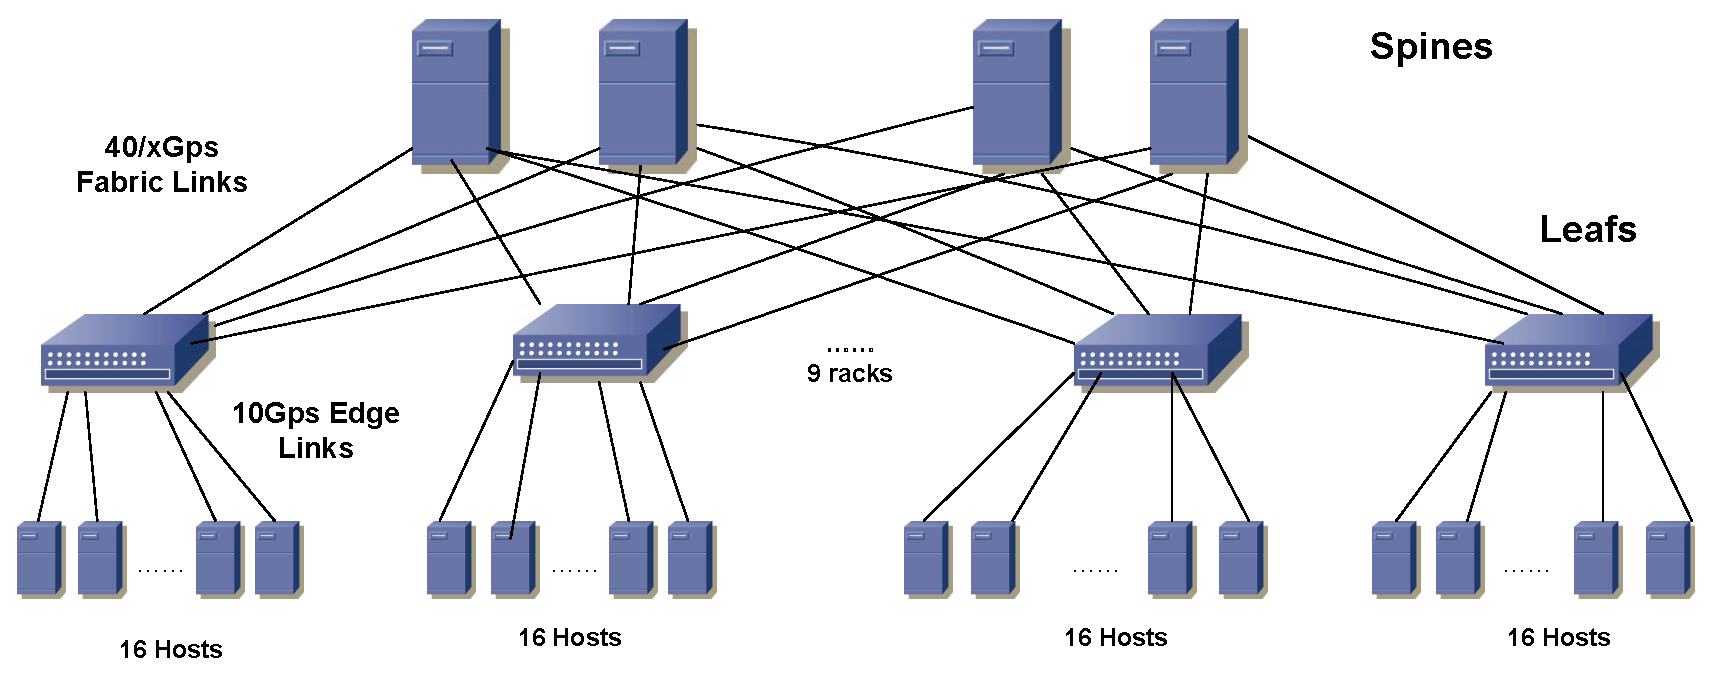
\includegraphics[width=0.8\columnwidth]{figures/FDRC/evaluation/spineleaf/spineleaf.eps}
  \caption{ns-2建立的数据中心拓扑}
\label{FDRC-DataCenterTop-fig}
\end{figure}

\textbf{数据中心流量特征}。
使用两种真实数据中心应用的流进行测试:网络搜索流和数据挖掘流\cite{DCTCP,LPD,pFabric}。
对于网络搜索应用,$70\%$的流小于$1MB$,超过$50\%$的流在100KB和1MB之间。
对于数据挖掘应用,超过80$\%$的流的小于$10KB$,超过90$\%$的数据量来自$4\%$的长流($>1MB$)。
在仿真实验中,本文使用不同的流到达速率来模拟不同的网络负载。
为了提高网络资源利用率,因而当前数据中心网络采取超额认购,所以在下面实验中,
改变叶子交换机和主干交换机之间的超额认购因子$x$来模拟此。

\textbf{性能指标}。
数据中心的数据流是有期限的流,带宽敏感的流,和需要高带宽的背景流的混合。
对于有显式截止期限的数据流,选择错过截止期限的流的百分比作为衡量策略针对这类数据流性能的指标。
对于短流,考虑流平均完成时间。
将FDRC与最先进的期限感知拥塞控制算法LPD-e\cite{LPD},D$^2$TCP\cite{D2TCP}和对期限不敏感的协议DCTCP\cite{DCTCP}进行比较。
对于未知截止期限的流,考虑流平均完成时间,
并将FDRC与pFabric\cite{pFabric},DCTCP\cite{DCTCP}和L$^2$DCT\cite{L2DCT}进行比较。

\textbf{FDRC的参数选择}。 
FDRC需要四个重要的参数。
根据\cite{D3},数据中心的流的期限在10ms到30ms之间来回震荡,所以选择$threshold\_lax$ = 30ms,$threshold\_tight$ = 10ms。
因子边界$DMAX$和$DMIN$可以根据(\ref{DMAX_DMIN_RANGE})设置。
在仿真实验中,$DMAX$是0.8,$DMIN$是0.3。


\subsubsection{时延敏感流优化}
在数据中心,网络搜索等时延敏感应用的流应在截止期限前传输完成,
如果流没有在截止期限前发送完毕,那么会影响应用的性能。
在本节,测试了FDRC对有截止期限流的优化。
实验中,假设流的截止期限服从统一分布,流的到达时间服从泊松分布,此外流的发送端和接收端都是随机选取的。
在数据中心,为了提高网络资源利用率,链路存在超额认购,
因此,变换叶子节点交换机和主干交换机链路的超额认购因子x,并重复各组实验100次。
在每组实验得到每组实验的最大值,最小值,和平均值,并在每组的error bar上进行标记。
同时,在每组实验中,使用DCTCP,D$^2$TCP,LPD-e与FDRC作对比。

\begin{figure}[h]
  \centering%
  \subcaptionbox{x=1\label{LPD_Motivation:subfig1}} %标题的长度,超过则会换行,如下一个小图。
    {\includegraphics[width=0.5\columnwidth]{figures/FDRC/evaluation/spineleaf/miss_deadline_1.eps}}%
  \subcaptionbox{x=4\label{LPD_Motivation:subfig2}}
      {\includegraphics[width=0.5\columnwidth]{figures/FDRC/evaluation/spineleaf/miss_deadline_3.eps}}
  \subcaptionbox{x=7\label{LPD_Motivation:subfig3}}%标题的长度,超过则会换行,如下一个小图。
    {\includegraphics[width=0.5\columnwidth]{figures/FDRC/evaluation/spineleaf/miss_deadline_7.eps}}%
  %\hspace{7em}%
  \subcaptionbox{x=10\label{LPD_Motivation:subfig4}}
      {\includegraphics[width=0.5\columnwidth]{figures/FDRC/evaluation/spineleaf/miss_deadline_10.eps}}
  \caption{使用网络搜索应用下的FDRC,LPD,D$^2$TCP之间错失期限的对比情形对比,流的期限是在10ms到30ms之间的统一分布}
  \label{fdrc-miss-spine-web-fig}
\end{figure}

\begin{figure}[h]
  \centering%
  \subcaptionbox{x=1\label{LPD_Motivation:subfig1}} %标题的长度,超过则会换行,如下一个小图。
    {\includegraphics[width=0.5\columnwidth]{figures/FDRC/evaluation/spineleaf/miss_deadline_4.eps}}%
  \subcaptionbox{x=4\label{LPD_Motivation:subfig2}}
      {\includegraphics[width=0.5\columnwidth]{figures/FDRC/evaluation/spineleaf/miss_deadline_6.eps}}
  \subcaptionbox{x=7\label{LPD_Motivation:subfig3}}%标题的长度,超过则会换行,如下一个小图。
    {\includegraphics[width=0.5\columnwidth]{figures/FDRC/evaluation/spineleaf/miss_deadline_8.eps}}%
  %\hspace{7em}%
  \subcaptionbox{x=10\label{LPD_Motivation:subfig4}}
      {\includegraphics[width=0.5\columnwidth]{figures/FDRC/evaluation/spineleaf/miss_deadline_9.eps}}
  \caption{使用数据挖掘应用下的FDRC,LPD,D$^2$TCP之间错失期限的对比情形对比,流的期限是在10ms到30ms之间的统一分布}
  \label{fdrc-miss-spine-data-fig}
\end{figure}


图\ref{fdrc-miss-spine-web-fig}表示的是网络搜索应用下的实验情况。
总体上,FDRC比D$^2$TCP和DCTCP性能好。
图\ref{fdrc-miss-spine-web-fig}(a) 显示的是超额认购系数x=1时,错失的流数目对比。
可以发现当网络负载从0.1到0.9时,使用DCTCP协议,错失期限流的数目在$3\%$$ \sim$$7\%$。
而使用D$^2$TCP,大约有$1\%$$ \sim $$2\%$的数据流错失期限。
使用FDRC,有$0.2\%$$ \sim $$1\%$的数据流错失期限。
使用LPD,大约有少于$0.5\%$的数据流错失期限。
图\ref{fdrc-miss-spine-web-fig}(b)显示的是超额认购系数x=4时,错失期限的流场景对比。
当网络负载从0.1到0.9时,使用DCTCP协议时,错失期限的流数目在$3.5\%$$ \sim$$7.5\%$,
D$^2$TCP大约有$1.5\%$$ \sim $$2.5\%$的数据流错失期限。
使用FDRC,有$0.7\%$$ \sim $$1.5\%$的数据流错失期限。
LPD下有少于$1\%$的数据流错失期限。
图\ref{fdrc-miss-spine-web-fig}(c)显示的是超额认购系数x=7时,错失期限的情形对比。
当网络负载从0.1到0.9时候,使用DCTCP协议时,错失期限的流的数目大约在$4\%$$ \sim$$8\%$。
而使用D$^2$TCP性能要提高一些,大约有$1\%$$ \sim $$3\%$的数据流错失期限。
使用FDRC,大约有$0.3\%$$ \sim $$2\%$比例的数据流错失期限。
使用LPD,大约有少于$1.5\%$的数据流错失期限。
图\ref{fdrc-miss-spine-web-fig}(d)显示的是超额认购系数x=10时,错失期限的对比。
当网络负载从0.1到0.9时候,使用DCTCP协议时,错失期限的流的数目大约在$3.5\%$$ \sim$$9\%$。
而使用D$^2$TCP性能要提高一些,大约有$1.5\%$$ \sim $$4\%$的数据流错失期限。
使用FDRC,大约有$0.7\%$$ \sim $$3\%$比例的数据流错失期限。
使用LPD,大约有少于$2\%$的数据流错失期限。
平均而言,对于网络搜索流而言,FDRC的流错失期限的比例是DCTCP的1/5,是D$^2$TCP的的1/2。
FDRC的性能仅次于LPD。


图\ref{fdrc-miss-spine-data-fig}表示的是数据挖掘流下的实验情况。
总的来看,FDRC依然是性能最好的。
图\ref{fdrc-miss-spine-data-fig}(a) 显示的是超额认购系数x=1时,错失期限的情形对比。
可以发现当网络负载从0.1到0.9时候,使用DCTCP协议时,错失期限的流的数目大约在$3.5\%$$ \sim$$6.5\%$。
而使用D$^2$TCP性能要提高一些,大约有$0.3\%$$ \sim $$0.8\%$的数据流错失期限。
使用FDRC,大约有$0.1\%$$ \sim $$0.3\%$比例的数据流错失期限。
使用LPD,大约有少于$0.3\%$的数据流错失期限。
图\ref{fdrc-miss-spine-data-fig}(b)显示的是超额认购系数x=4时,错失期限的情形对比。
当网络负载从0.1到0.9时候,使用DCTCP协议时,错失期限的流的数目大约在$4\%$$ \sim$$8\%$。
而使用D$^2$TCP性能要提高一些,大约有$0.5\%$$ \sim $$2\%$的数据流错失期限。
使用FDRC,大约有$0.3\%$$ \sim $$1\%$比例的数据流错失期限。
使用LPD,大约有少于$0.5\%$的数据流错失期限。
图\ref{fdrc-miss-spine-data-fig}(c)显示的是超额认购系数x=7时,错失期限的情形对比。
当网络负载从0.1到0.9时候,使用DCTCP协议时,错失期限的流的数目大约在$4\%$$ \sim$$8.5\%$。
而使用D$^2$TCP性能要提高一些,大约有$1\%$$ \sim $$3.5\%$的数据流错失期限。
使用FDRC,大约有$0.4\%$$ \sim $$0.9\%$比例的数据流错失期限。
使用LPD,大约有少于$0.7\%$的数据流错失期限。
图\ref{fdrc-miss-spine-data-fig}(d)显示的是超额认购系数x=10时,错失期限的情形对比。
当网络负载从0.1到0.9时候,使用DCTCP协议时,错失期限的流的数目大约在$4.5\%$$ \sim$$9\%$。
而使用D$^2$TCP性能要提高一些,大约有$0.5\%$$ \sim $$4\%$的数据流错失期限。
使用FDRC,大约有$0.4\%$$ \sim $$1\%$比例的数据流错失期限。
使用LPD,大约有少于$1\%$的数据流错失期限。


平均而言,对于数据挖掘场景下,FDRC的表现和web搜索场景下基本相似。
使用FDRC导致流错失期限的比例是DCTCP的1/5,是D$^2$TCP的的1/2。
FDRC的性能仅次于LPD。
认为,虽然FDRC的性能不及LPD,但是LPD需要预先得知流的大小和期限,
而在数据中心中,很多应用数据流期限和流大小是很难预先得知的,
因此FDRC的应用范围要比LPD广泛,尽管FDRC有一些性能损失。

\begin{figure}[h]
\centering
\subcaptionbox{紧急期限}
 {\includegraphics[width=0.32\columnwidth]{figures/FDRC/evaluation/spineleaf/miss_deadline_tcp_tight.eps}}
\subcaptionbox{中等期限}
{\includegraphics[width=0.32\columnwidth]{figures/FDRC/evaluation/spineleaf/miss_deadline_tcp_mild.eps}}
\subcaptionbox{松弛期限}
{\includegraphics[width=0.32\columnwidth]{figures/FDRC/evaluation/spineleaf/miss_deadline_tcp_lax.eps}}
\caption{网络搜索应用的场景下,FDRC 和 LPD, D$^2$TCP, DCTCP错失期限对比。流的期限服从指数分布}
\label{fdrc-miss-spine-data-fig}
\end{figure}

在数据中心中,并不是所有的流都存在明确期限,
数据中心的数据流往往是有期限的流,没有期限的短流,背景流的混合。
在本组实验中,把网络搜索流平均分成两组:第一组,设置显示的期限;第二组,是背景流,没有显式的期限。
在仿真实验中,设置三组期限:紧急期限(10ms),中等期限(20ms),松弛期限(30ms)。
设定所有流的到达服从泊松分布,数据流的源端和目的端都是随机选择的。
图\ref{fdrc-miss-spine-data-fig}是实验结果。

图\ref{fdrc-miss-spine-data-fig}(a)显示的是紧急期限(10ms)情形下流错失期限的情形对比。
发现使用DCTCP大约有$1\%$$\sim$$6\%$的流错失期限。
使用D$^2$TCP大约有$1\%$$\sim$$3\%$的流错失期限。
使用FDRC大约有$1\%$$\sim$$2.5\%$的流错失期限。
FDRC比DCTCP和D$^2$TCP性能提高1$\times$和$10\%$。
图\ref{fdrc-miss-spine-data-fig}(b)显示的是中等期限(20ms)情形下流错失期限的情形对比。
发现使用DCTCP大约有$0.5\%$$\sim$$5\%$的流错失期限。
使用D$^2$TCP大约有$1\%$$\sim$$2.5\%$的流错失期限。
使用FDRC大约有$1\%$$\sim$$2\%$的流错失期限。
FDRC比DCTCP和D$^2$TCP性能提高2$\times$和$20\%$。
图\ref{fdrc-miss-spine-data-fig}(c)显示的是松弛期限(30ms)情形下流错失期限的情形对比。
发现使用DCTCP大约有$1\%$$\sim$$4\%$的流错失期限。
使用D$^2$TCP大约有$0.5\%$$\sim$$1.6\%$的流错失期限。
使用FDRC大约有$0.5\%$$\sim$$1\%$的流错失期限。
FDRC比DCTCP和D$^2$TCP性能提高4$\times$和$40\%$。
平均来看,对于有期限的流的优化,FDRC的性能比DCTCP提高大约4倍,比D$^2$TCP的性能提高大约$30\%$。




\subsubsection{流平均完成时间对比}
在多瓶颈链路场景下,最小化流平均完成时间和多染色问题是等价的\cite{COLOR}。
在单条链路上,最短流优先(Shortest-Flow-First,简称SFF)策略是最优策略。
FDRC近似的实现了最短流优先策略,因此对流平均时间的优化较好。


\begin{figure}[h]
\centering
\subcaptionbox{流平均完成时间}
 {\includegraphics[width=0.32\columnwidth]{figures/FDRC/evaluation/spineleaf/FCT_SEARCH_average.eps}}
\subcaptionbox{(500KB,+$\infty$)}
{\includegraphics[width=0.32\columnwidth]{figures/FDRC/evaluation/spineleaf/FCT_SEARCH_large.eps}}
\subcaptionbox{(0,100KB)}
{\includegraphics[width=0.32\columnwidth]{figures/FDRC/evaluation/spineleaf/FCT_SEARCH_large.eps}}
\caption{网络搜索应用的场景下,FDRC,DCTCP,L$^2$DCT,pFabric下的流平均完成时间对比。图(a)展示的是流平均完成时间对比情况;图(b)显示的是长流的流平均完成时间;图(c)显示的是短流的平均完成时间}
\label{fdrc-fct-spine-search-5-fig}
\end{figure}

图\ref{fdrc-fct-spine-search-5-fig}显示的是网络搜索应用下的流平均完成时间结果对比。
图\ref{fdrc-fct-spine-search-5-fig}(a)展示的是流平均完成时间的整体情形。
可以看到当网络的负载从$0.1$$\sim$$0.9$时,使用DCTCP,流的平均完成时间$0.01s$$\sim$$0.05s$。
优化流平均完成时间的方法L$^2$DCT,性能要更好,使用L$^2$DCT,流的平均完成时间在$0.01s$$\sim$$0.03s$。
总体看L$^2$DCT的性能比DCTCP要提高1$\times$。
使用FDRC,流的平均完成时间要更加好,当网络负载从$0.1$$\sim$$0.9$时,
流的平均完成时间在$0.005s$$\sim$$0.025s$。
pFabric是当前的优化流平均完成时间的最优策略,pFabric的流平均完成时间在$0.003s$$\sim$$0.023s$之间。
pFabric的性能比FDRC要高$20\%$。
FDRC的性能比L$^2$DCT提高$30\%$。
图\ref{fdrc-fct-spine-search-5-fig}(b)展示的是长流平均完成时间的结果。
可以看到当网络负载从$0.1$$\sim$$0.9$时,使用DCTCP流平均完成时间在$0.03s$$\sim$$0.15s$。
针对流平均完成时间的方法L$^2$DCT,表现的要好一些,使用L$^2$DCT,流的平均完成时间在$0.02s$$\sim$$0.05s$
总体看L$^2$DCT的性能比DCTCP要提高1$\times$。
pFabric是当前的优化流平均完成时间的最优策略,pFabric的流平均完成时间在$0.005s$$\sim$$0.02s$之间。
pFabric的性能比FDRC要高$20\%$。
FDRC的性能比L$^2$DCT提高$25\%$。
图\ref{fdrc-fct-spine-search-5-fig}(c)展示的是短流平均完成时间的整体情况。
可以看到当网络的负载从$0.1$$\sim$$0.9$时,使用DCTCP的流的平均完成时间在$0.01s$$\sim$$0.05s$。
使用L$^2$DCT,流的平均完成时间在$0.01s$$\sim$$0.03s$,使用FDRC,流的平均完成时间要更加好。
pFabric的流平均完成时间在$0.003s$$\sim$$0.023s$之间。
pFabric的性能比FDRC要高$20\%$。
而FDRC的性能比L$^2$DCT提高$30\%$。


\begin{figure}[h]
\centering
\subcaptionbox{流平均完成时间}
 {\includegraphics[width=0.32\columnwidth]{figures/FDRC/evaluation/spineleaf/FCT_DATA_average.eps}}
\subcaptionbox{(500KB,+$\infty$)}
{\includegraphics[width=0.32\columnwidth]{figures/FDRC/evaluation/spineleaf/FCT_DATA_large.eps}}
\subcaptionbox{(0,100KB)}
{\includegraphics[width=0.32\columnwidth]{figures/FDRC/evaluation/spineleaf/FCT_DATA_large.eps}}
\caption{数据挖掘应用的场景下,FDRC,DCTCP,L$^2$DCT,pFabric下的流平均完成时间对比。图(a)展示的是平均的流完成时间对比情况;图(b)显示的是流大小大于500KB时的情形;图(c)显示的是短流的平均完成时间}
\label{fdrc-fct-spine-data-5-fig}
\end{figure}


图\ref{fdrc-fct-spine-data-5-fig}显示的是数据挖掘应用下的流平均完成时间的对比。
图\ref{fdrc-fct-spine-data-5-fig}(a)展示的是流平均完成时间的整体情况。
可以看到当网络的负载从$0.1$$\sim$$0.9$时,使用DCTCP的流的平均完成时间在$0.18s$$\sim$$0.25s$。
针对流平均完成时间的方法L$^2$DCT,表现的要好一些,使用L$^2$DCT,流的平均完成时间在$0.11s$$\sim$$0.15s$
当网络负载从$0.1$$\sim$$0.9$时,使用FDRC的流平均完成时间在$0.008s$$\sim$$0.14s$。
使用pFabric的流平均完成时间在$0.05s$$\sim$$0.08$之间。
pFabric的性能比FDRC要高$30\%$。
FDRC的性能比L$^2$DCT提高$12\%$。
图\ref{fdrc-fct-spine-data-5-fig}(b)展示的是长流平均完成时间的结果。
可以看到当网络的负载从$0.1$$\sim$$0.9$时,使用DCTCP的流的平均完成时间在$0.2s$$\sim$$0.3s$。
针对流平均完成时间的方法L$^2$DCT,表现的要好,使用L$^2$DCT,流的平均完成时间在$0.18s$$\sim$$0.22s$
使用FDRC,流的平均完成时间在$0.14s$$\sim$$0.18s$,使用pFabric的流平均完成时间在$0.11s$$\sim$$0.15s$之间。
FDRC的性能比L$^2$DCT提高$15\%$。
图\ref{fdrc-fct-spine-data-5-fig}(c)展示的是短流平均完成时间的情形,
结果与图\ref{fdrc-fct-spine-data-5-fig}(a)以及图\ref{fdrc-fct-spine-data-5-fig}(b)基本相同。

因此总体看FDRC的性能比DCTCP和L$^2$DCT要高,但是不如pFabric。
但是pFabric是调度的方法,需要修改交换机的硬件,FDRC用当前数据中心的硬件就能实现,
因此,适用的场景更广。

\begin{figure}[h]
\centering
\subcaptionbox{流平均完成时间}
 {\includegraphics[width=0.32\columnwidth]{figures/FDRC/evaluation/spineleaf/fct.eps}}
\subcaptionbox{(500KB,+$\infty$)}
{\includegraphics[width=0.32\columnwidth]{figures/FDRC/evaluation/spineleaf/large_fct.eps}}
\subcaptionbox{(0,100KB)}
{\includegraphics[width=0.32\columnwidth]{figures/FDRC/evaluation/spineleaf/small_fct.eps}}
\caption{网络搜索流量下,FDRC,DCTCP,L$^2$DCT,pFabric的标准化的流平均时间对比。 注意在图(c)中,DCTCP没有出现其中,因为DCTCP的平均流完成时间太长,因此并没有画出}
\label{fdrc-fct-spine-fct-factor-fig}
\end{figure}

图\ref{fdrc-fct-spine-fct-factor-fig}是网络搜索流量, 
变换链路的超额认购系数的FDRC,DCTCP,L$^2$DCT,pFabric,标准化的流平均时间的对比。
图\ref{fdrc-fct-spine-fct-factor-fig}(a)描述的是流平均完成时间的整体情况。
发现,当超额认购系数从5增加到30时,DCTCP的流平均完成时间从5增加到70。
L$^2$DCT的性能比DCTCP强,使用L$^2$DCT,流平均完成时间在3到22之间,L$^2$DCT的性能大约是DCTCP的3$\times$。
FDRC的性能优于L$^2$DCT,使用FDRC的流平均完成时间在3到17之间。
FDRC的性能比L$^2$DCT提高$30\%$。
近似最优的策略pFabric的性能最好,使用pFabric下的流平均完成时间在2到10之间。FDRC的性能比之差$30\%$。
图\ref{fdrc-fct-spine-fct-factor-fig}(b)描述的是流大小在(500KB,+$\infty$)时,流平均完成时间的整体情况。
发现,对于这些长流,当超额认购系数从5增加到30时,DCTCP的流平均完成时间从5增加到120。
使用L$^2$DCT,流平均完成时间在3到74之间,L$^2$DCT的性能比DCTCP提高大约$40\%$。
FDRC的性能优于L$^2$DCT,使用FDRC的流平均完成时间在3到40之间。
FDRC的性能比L$^2$DCT提高1$\times$。
近似最优的策略pFabric的性能最好,使用pFabric下的流平均完成时间在2到20之间。
FDRC的性能比之差$30\%$。
图\ref{fdrc-fct-spine-fct-factor-fig}(c)描述的是短流的流平均完成时间的整体情形。
实验的结果和前面两组基本类似。

\subsection{真实环境下的测试床测试}
\begin{figure}[H] 
  \centering
  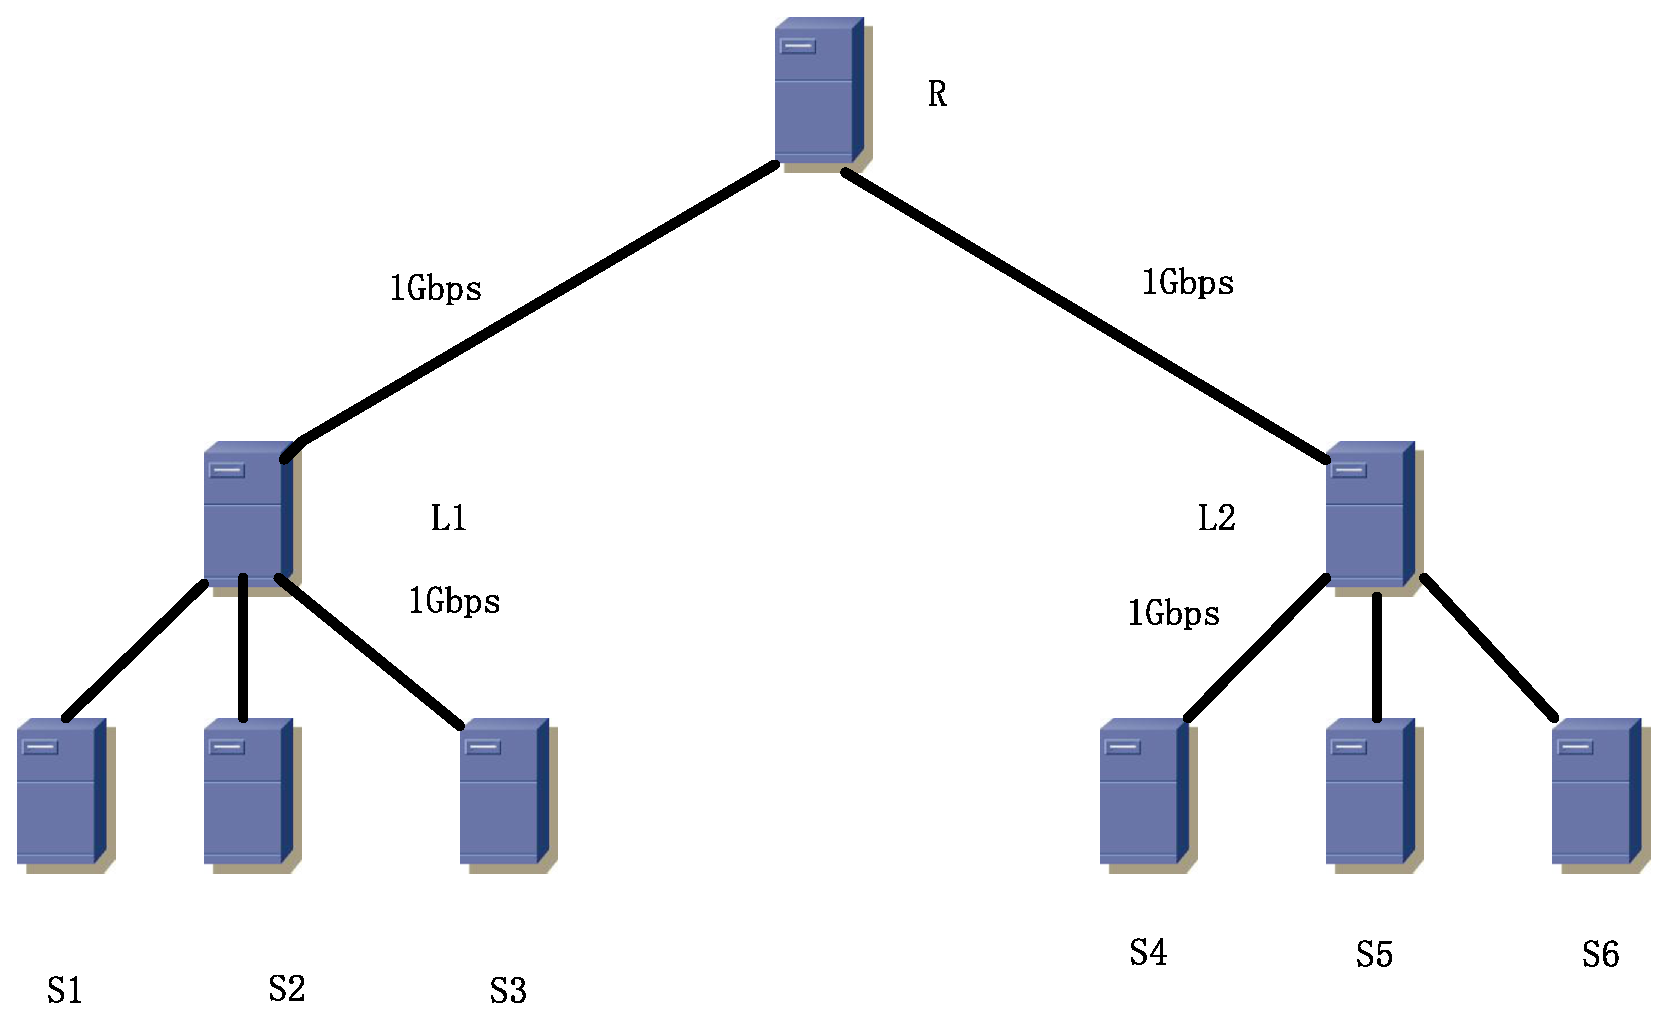
\includegraphics[width=0.8\columnwidth]{figures/FDRC/evaluation/Realtest/testbed.eps}
  \caption{小型数据中心测试床}
\label{fdrc-testbed-fig}
\end{figure}
为了测试FDRC在真实环境下的性能,基于DCTCP的代码\cite{DCTCPcode},在Linux内核3.2.61的平台下实现了D$^2$TCP,L$^2$DCT,LPD。
在实验中,使用Linux系统当作交换机,当作交换机的Linux系统运行的是FreeBSD 9.1,系统上安装了DummyNet\cite{dummynet},改进了
DummyNet来进行数据包的标记和线速的转发。
因为硬件数目的限制,建立了小型的树状的拓扑,拓扑有3个交换机,6个机器,拓扑的结构如图\ref{fdrc-testbed-fig}所示。

\subsubsection{带宽测试}
使用FDRC,流开始有最高的优先级,随着时间的流逝,流的优先级开始降低。
在本组中,测试真实环境下FDRC的带宽等的性能。
在的测试实验中,设置$DMAX=0.8$,$DMIN=0.3$,设置$threshold\_lax$= 200ms,阈值$threshold\_tight$= 100ms,交换机的队列$K=40KB$。
启动4条数据流,$flow_1$从$S_1$启动,启动时间为$t=0s$,$flow_2$从$S_2$启动,启动时间为$t=0.3s$,$flow_3$从$S_3$启动,启动时间为$t=0.4s$,$flow_4$从$S_4$启动,启动时间为$t=0.5s$,所有流的目的地都是机器R。

\begin{figure}[h]
\centering
\subcaptionbox{4条流带宽}
 {\includegraphics[width=0.48\columnwidth]{figures/FDRC/evaluation/Realtest/rate.eps}}
\subcaptionbox{交换机队列长度}
{\includegraphics[width=0.48\columnwidth]{figures/FDRC/evaluation/Realtest/realqueue.eps}}
\caption{(a) 显示了四条流的带宽. (b) 显示了交换机的队列长度}
\label{fdrc-testbed-bandwidt-queue}
\end{figure}
图\ref{fdrc-testbed-bandwidt-queue}展示的是流完成时间对比。
从图\ref{fdrc-testbed-bandwidt-queue}(a)发现,使用FDRC协议,流开始的平均带宽最高,随着时间的流逝,流的带宽开始下降,
最后,当流的持续时间大于200ms时,流达到最低优先级,最终,所有的流有相同的优先级,它们共享链路带宽。
图\ref{fdrc-testbed-bandwidt-queue}(b)是队列,可以看到,队列长度始终保持在比较低的水平上,设置的$K=40KB$,因此
交换机的队列在40KB波动。
因此使用FDRC方法,能够在维持链路高带宽的基础上同时维持队列维持在比较短的水平。





\subsubsection{错失期限测试}
在本小节,测试当数据中心中有延迟敏感的数据流FDRC的性能。
在实验中,首先,每个机器$S_i$和随机的选取一台机器建立TCP连接。
每个TCP连接持续T分钟。
在T分钟中,$S_i$将会发送短的数据流给接收端。
T分钟过后,这台机器$S_i$会再随机选择一台机器,然后重复这个过程。
在这组实验中,设置$DMAX=0.8$,$DMIN=0.3$,设置$threshold\_lax$= 200ms,阈值$threshold\_tight$= 100ms,
设置流的期限在100ms到200ms之间,并且重复这个过程100次,为了进行对比,同样实现了D$^2$TCP,LPD
和DCTCP,变化数据包的大小,最终的实验结果如图\ref{fdrc-qmin-fig}所示。

从图\ref{fdrc-qmin-fig}看到,整体上,FDRC的性能好于DCTCP,D$^2$TCP,但是比LPD要差。
当数据包大小在$50KB$时,FDRC错失流的比例平均为$0.3\%$,当数据包大小为$100KB$时,FDRC错失流的比例平均为$0.5\%$。
当数据包大小为$150KB$时,FDRC错失流的比例平均为$1\%$,当数据包大小为$200KB$时,FDRC错失流的比例平均为$1.2\%$。
FDRC的性能整体比DCTCP提升3$\times$,比D$^2$TCP提升$30\%$。

\subsubsection{流平均完成时间优化测试}
在本小节,测试FDRC对流完成时间的优化。
在实验中,首先,每个机器$S_i$和随机的选取一台机器建立TCP连接。
每个TCP连接持续T分钟。
在T分钟中,$S_i$将会发送短的数据流给接收端。
T分钟过后,这台机器$S_i$会再随机选择一台机器,然后重复此过程。
在这组实验中,设置$DMAX=0.8$,$DMIN=0.3$,设置$threshold\_lax$= 200ms,阈值$threshold\_tight$= 100ms,
重复这个过程100次,为了进行对比,同样实现了D$^2$TCP,LPD
和DCTCP,变化数据包的大小,最终的实验结果如图\ref{fdrc-fct-fig}所示。

从图\ref{fdrc-fct-fig}看到,整体上,FDRC的性能好于DCTCP,L$^2$DCT,但是比LPD要差。
当数据包大小在$50KB$时,FDRC的流平均完成时间在0.5ms;当数据包大小在$100KB$时,FDRC的流平均完成时间在1ms;
当数据包大小在$150KB$时,FDRC的流平均完成时间在2.5ms;当数据包大小在$200KB$时,FDRC的流平均完成时间在3ms。

\begin{figure}
\begin{minipage}{0.5\textwidth}
  \centering
  \includegraphics[width=0.7\columnwidth]{figures/FDRC/evaluation/Realtest/miss_deadline_.eps}
  \caption{错失期限的流的比例}
  \label{fdrc-qmin-fig}
\end{minipage}
\begin{minipage}{0.5\textwidth}
  \centering
  \includegraphics[width=0.7\columnwidth]{figures/FDRC/evaluation/Realtest/fct_.eps}
  \caption{流平均完成时间}
  \label{fdrc-fct-fig}
\end{minipage}
\end{figure}

\section{本章总结}

在本章中,把流持续时间引入到惩罚函数的计算中。
本文通过设置适当的阈值,紧急的流比背景流获得更多带宽,从而在截止期限之前完成。
基于此,本文提出基于流持续时间的速率控制机制(Flow Duration Time Rate Control,简称FDRC),并且对FDRC建模。
实验发现FDRC性能比D$^2$TCP和L$^2$DCT高30$\%$。
尽管FDRC在仿真和真实环境中性能都很好,但是本章未对FDRC的稳定性等进行讨论。





